% -------------------------------------------------------------------------------------
% This is a general template file for publish an article for Revista Colombiana de Estad�stica
% *************************************************************************************

\documentclass[english]{revcoles}


 
% //// --------------------------------------------------------------------------------
\begin{document}

\title[maintitle = Title in English,
       secondtitle = Title in Spanish,
       shorttitle = Short title in English
]

\begin{authors}
\author[firstname = Name,
        surname = Last Name,
        numberinstitution = 1,
        affiliation = Institution and Department,
        email = email]
\author[firstname = Name,
        surname = Last Name,
        numberinstitution = 2,
        affiliation = Institution and Department,
        email = email]
\author[firstname = Name,
        surname = Last Name,
        numberinstitution = 3,
        affiliation = Institution and Department,
        email = email]
\end{authors}

\begin{institutions}
     \institute[subdivision = {Department or School},
                division = Faculty or Division,
                institution = University or Institution,
                city = City,
                country = Country]
     \institute[subdivision = {Department or School},
                division = Faculty or Division,
                institution = University or Institution,
                city = City,
                country = Country]
     \institute[subdivision = {Department or School},
                division = Faculty or Division,
                institution = University or Institution,
                city = City,
                country = Country]
\end{institutions}

\begin{mainabstract}
 Insert your abstract here.
\keywords{First keyword, second keyword, other keywords }
\end{mainabstract}

\begin{secondaryabstract}
Inserte su resumen en aqu�.
%
\keywords{Palabra clave uno, palabra clave dos, otras palabras clave}
\end{secondaryabstract}

\section{Introduction}


\section{Section title} \label{sec:1}

Your text comes here.

\begin{table}[!h]
\caption{Please write your table caption here}\label{table1}
\centering {\small
\begin{tabular}{ccrc}\hline
x   & y   & z   &  w \\ \hline
x1  & y1  & z1  & w1  \\
x2  & y2  & z2  & w2  \\
x3  & y3  & z3  & w3  \\
x4  & y4  & z4  & w4  \\ \hline
\end{tabular}}
\end{table}


\begin{table}[!htb]
\centering\small \caption{Please write your table caption here}\label{table2}
\renewcommand{\arraystretch}{1.5}
\begin{tabular}{ccccc}\hline
\parbox[c][0.9\height]{18mm}{\centering\smallskip Source of\\Variation\smallskip} &%
\parbox[c][0.9\height]{25mm}{\centering\smallskip Degrees of\\Freedom\smallskip} &%
\parbox[c][0.9\height]{16mm}{\centering\smallskip Sum of \\Squares\smallskip} &%
\parbox[c][0.9\height]{15mm}{\centering\smallskip Mean\\Square\smallskip}& F\\\hline
Model & $p+r-2$&$SCM^*$&$CMM^*$&$FG^*=\frac{CMM^*}{CME}$\\ %\hline
Fixed Effects & $p-1$&$SCMF^*$&$CMMF^*$&$FF=\frac{CMMF^*}{CME}$\\ \hline
\end{tabular}
\end{table}

\section{Section title} \label{sec:2}
\begin{figure}[htb]
  \centering
  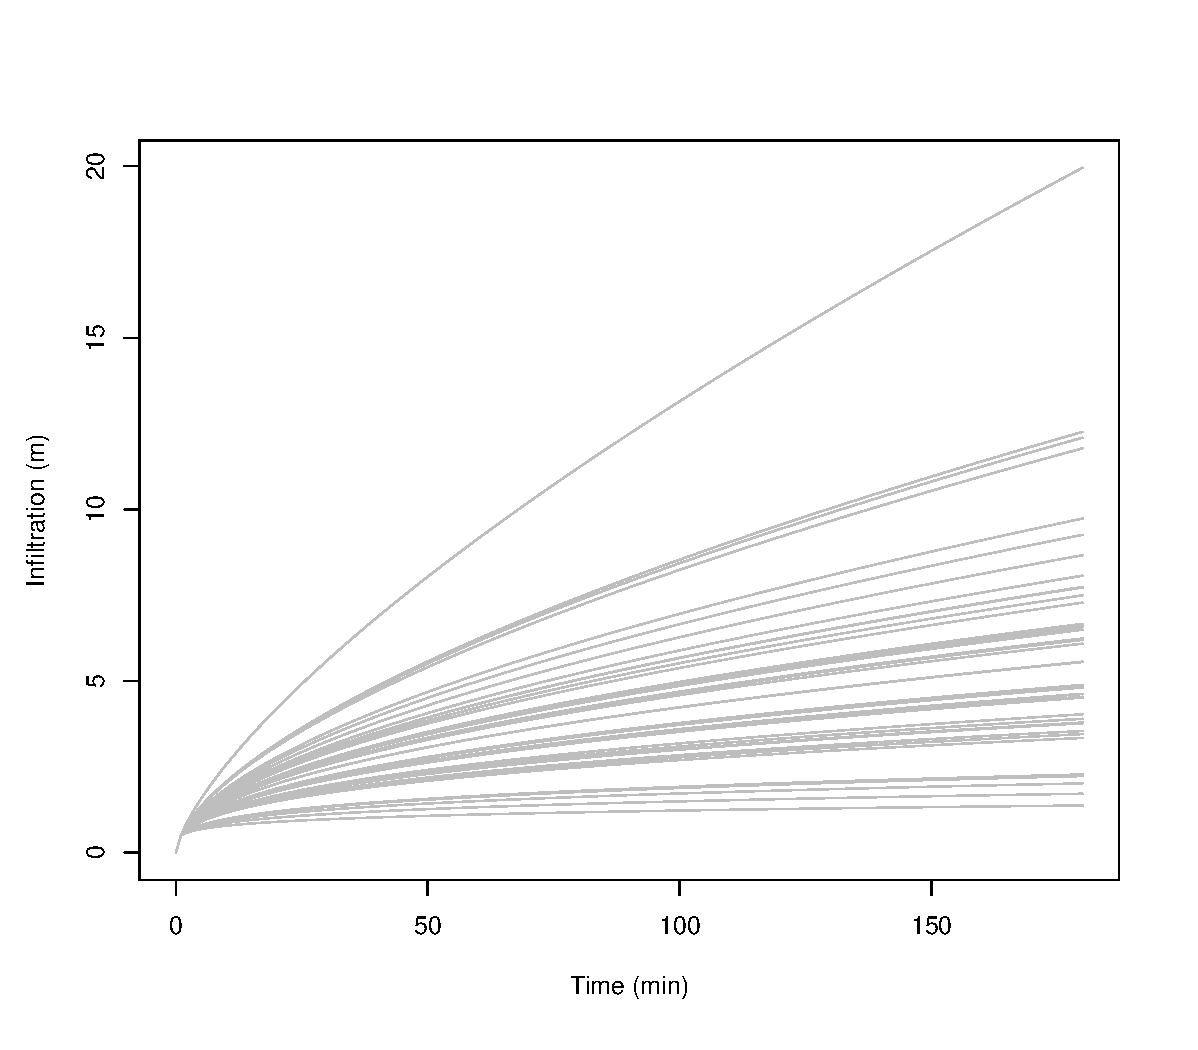
\includegraphics[scale=0.4]{graph_example.eps}
  \caption{Please write your figure caption here}\label{figure1}
\end{figure}

\begin{itemize}

\item The model proposed by \citeasnoun{Dodge-85}\dots
\item Such is shown in  \citeasnoun{Conover-81}  \dots
\item The simulation study was carried out by using \citeasnoun{R} \dots

\end{itemize}

\begin{equation}\label{equ1}
    y=W\mu+Z\theta+e
\end{equation}

\begin{equation}\label{equ2}
\begin{bmatrix}
W'R^{-1}W&W'R^{-1}Z\\
Z'R^{-1}W&Z'R^{-1}Z+D^{-1}
\end{bmatrix}
\begin{bmatrix}
\mu \\ \theta
\end{bmatrix}=
\begin{bmatrix}
W'R^{-1}y\\
Z'R^{-1}y
\end{bmatrix}
\end{equation}

\section{Conclusions}

\section{Acknowledgements}
If you'd like to thank anyone, place your comments here.

% BibTeX users please use
    \bibliography{references}

    \appendix% !don't modify this line�

\end{document}

